\section{收敛方式的比较}
\label{sec:rvconv-comparison}

三种收敛控制的对象不同：几乎必然收敛管每条记录的最终行为，依概率收敛管每一项超差事件的大小，$L^{p}$收敛管误差的平均大小。上一节的例子已经显示它们并不等价。哪些要求能推出另一些？推不出时，缺的是哪一种控制？

在一般测度空间上，几乎处处收敛推出依测度收敛需要总测度有限，$L^{r}$收敛推出较低阶的$L^{p}$收敛也需要总测度有限。概率空间的总质量为一，这两个条件自动满足，于是得到下面三条蕴含关系。

\begin{theorem}[收敛方式的蕴含关系]
\label{thm:rvconv-implications}
设$X_n,X$是同一概率空间上的实随机变量，$1\leq p<r<\infty$。
\begin{enumerate}
 \item 若$X_n\xrightarrow{\mathrm{a.s.}}X$，则$X_n\xrightarrow{\mathbb{P}}X$。
 \item 若$X_n\xrightarrow{L^{p}}X$，则$X_n\xrightarrow{\mathbb{P}}X$；更具体地，对每个$\varepsilon>0$，
 \begin{equation}
  \mathbb{P}\bigl(\lvert X_n-X\rvert>\varepsilon\bigr)\leq\frac{\mathbb{E}\bigl[\lvert X_n-X\rvert^{p}\bigr]}{\varepsilon^{p}} .
  \label{eq:rvconv-markov-lp}
 \end{equation}
 \item 若$X_n\xrightarrow{L^{r}}X$，则$X_n\xrightarrow{L^{p}}X$；更具体地，
 \begin{equation}
  \lVert X_n-X\rVert_{p}\leq\lVert X_n-X\rVert_{r} .
  \label{eq:rvconv-lp-monotone}
 \end{equation}
\end{enumerate}
\end{theorem}

\begin{proof}
第1条。固定$\varepsilon>0$，令
\[
 G_N=\bigcup_{n\geq N}\bigl\{\lvert X_n-X\rvert>\varepsilon\bigr\},
\]
即从第$N$项起至少超差一次的记录。$G_N$随$N$递减。若$\omega$属于每一个$G_N$，则$\omega$上超差发生无穷多次，$X_n(\omega)\not\to X(\omega)$；所以$\bigcap_NG_N\subseteq\{X_n\not\to X\}$，它的概率为零。

概率测度对递减事件列连续（第~\ref{chap:probability-spaces}章），这里用到总质量有限：
\[
 \mathbb{P}(G_N)\to\mathbb{P}\Bigl(\bigcap_NG_N\Bigr)=0 .
\]
而第$N$项的超差事件含于$G_N$，它的概率不超过$\mathbb{P}(G_N)$，也趋于零。

第2条。超差事件含于$p$次幂的超差事件：
\[
 \{\lvert X_n-X\rvert>\varepsilon\}\subseteq\{\lvert X_n-X\rvert^{p}\geq\varepsilon^{p}\} .
\]
对非负随机变量$\lvert X_n-X\rvert^{p}$和阈值$\varepsilon^{p}$用Markov不等式（第~\ref{chap:tail-probabilities}章），即得式~\eqref{eq:rvconv-markov-lp}。右边趋于零，左边也趋于零。

第3条。第~\ref{chap:random-variable-moments}章由Jensen不等式证明了绝对矩开相应次方后随阶数单调增加：对任意随机变量$V$，
\[
 \bigl(\mathbb{E}[\lvert V\rvert^{p}]\bigr)^{1/p}\leq\bigl(\mathbb{E}[\lvert V\rvert^{r}]\bigr)^{1/r} .
\]
取$V=X_n-X$即得式~\eqref{eq:rvconv-lp-monotone}。
\end{proof}

第1条证明中的$G_N$把整个尾段的超差合在一起。几乎必然收敛控制的正是这个尾段的并，依概率收敛只控制其中一项，前者自然更强；第~\ref{sec:rvconv-infinitely-often}小节会把这一观察写成等价条件。第3条在一般测度空间上要多出一个因子，即总测度的$1/p-1/r$次幂，概率空间中这个因子是$1$。

\paragraph{用累计最大值核对}
取$n=10$，$\varepsilon=0.1$。精确的超差概率是$0.9^{10}\approx0.349$。由式~\eqref{eq:rvconv-markov-lp}，用平均绝对误差$1/11$与均方误差$2/132$分别得到上界
\[
 \frac{1/11}{0.1}\approx0.909,\qquad \frac{2/132}{0.01}\approx1.52 .
\]
两个界都成立，后者大于$1$而没有信息。式~\eqref{eq:rvconv-lp-monotone}也可以直接核对：
\[
 \lVert1-M_{10}\rVert_{1}\approx0.0909\leq\lVert1-M_{10}\rVert_{2}=\sqrt{2/132}\approx0.123 .
\]

\paragraph{逆命题的反例}
三条蕴含关系都不能反过来。表~\ref{tab:rvconv-examples}汇总了贯穿例子的收敛情况，其中独立示性变量$\xi_n$取$p_n=1/n$，它不几乎必然收敛这一点要到第~\ref{sec:rvconv-borel-cantelli}小节才能证明。

\begin{BookInlineTable}
 \centering
 \begin{tabular}{@{}lcccc@{}}
  \toprule
  随机变量列 & 几乎必然 & 依概率 & $L^{1}$ & $L^{2}$ \\
  \midrule
  $M_n\to1$ & 是 & 是 & 是 & 是 \\
  移动区块$B_n\to0$ & 否 & 是 & 是 & 是 \\
  $\xi_n\to0$，$p_n=1/n$ & 否 & 是 & 是 & 是 \\
  $Z_n=\sqrt n\,\mathbf{1}_{\{U<1/n\}}\to0$ & 是 & 是 & 是 & 否 \\
  $Y_n=n\,\mathbf{1}_{\{U<1/n\}}\to0$ & 是 & 是 & 否 & 否 \\
  \bottomrule
 \end{tabular}
 \caption{贯穿例子在四种意义下是否收敛。}
 \label{tab:rvconv-examples}
\end{BookInlineTable}

表中的“否”来自两种不同的缺陷。第一种是缺少尾部控制：$Y_n$和$Z_n$的超差概率$1/n$趋于零，每条记录最终也归于零，但偶尔出现的误差越来越大，大到足以维持平均。依概率收敛与几乎必然收敛都只看误差是否超过$\varepsilon$，对超出多少一无所知，所以推不出$L^{p}$收敛。

第二种是缺少整列的逐样本控制：$B_n$和$\xi_n$的误差只取$0$或$1$，平均误差和超差概率一起趋于零，但超差事件在$\Omega$上不断移动或独立地重新出现，每条记录（或几乎每条记录）上都无穷多次超差。$L^{p}$收敛与依概率收敛都是逐项的要求，管不到同一条记录在不同时刻的表现，所以推不出几乎必然收敛。

\begin{BookInlineFigure}
 \centering
 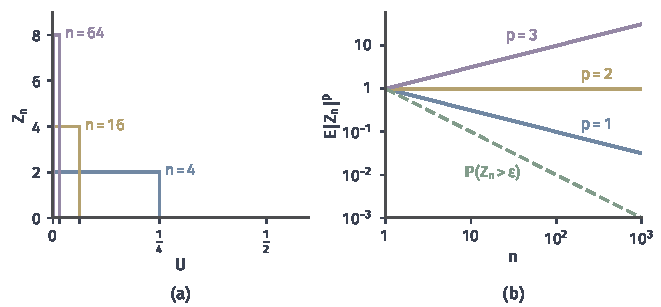
\includegraphics[width=112mm]{figures/07-probability/03-probability-limits/matplotlib/rvconv-power-spikes/figure.pdf}
 \caption{稀有大值$Z_n=\sqrt n\,\mathbf{1}_{\{U<1/n\}}$。(a)$Z_n$作为$U$的函数，$n=4,16,64$：高为$\sqrt n$、宽为$1/n$的矩形。(b)双对数坐标下的精确矩$\mathbb{E}[\lvert Z_n\rvert^{p}]=n^{p/2-1}$，$p=1,2,3$（蓝、黄、紫），绿色虚线是超差概率$1/n$（$0<\varepsilon<1$）。}
 \label{fig:rvconv-power-spikes}
\end{BookInlineFigure}

图~\ref{fig:rvconv-power-spikes}把第一种缺陷画出来。(a)中矩形越来越窄、越来越高；$p$阶矩是$\lvert Z_n\rvert^{p}$下方的面积，宽度按$1/n$缩小，高度的$p$次幂按$n^{p/2}$增长。(b)中各条直线的斜率$p/2-1$表明两者谁占上风：$p<2$时宽度胜出，$p=2$时恰好持平，$p>2$时高度胜出。超差概率的斜率是$-1$，它对高度完全不敏感。

\paragraph{较高阶与较低阶}
$Z_n$还说明第3条不能反过来：$L^{1}$收敛推不出$L^{2}$收敛。较低阶的平均把大误差压得较轻，较高阶的平均把它放得较重，所以控制高阶误差的要求更强。

\paragraph{两种收敛同时成立时}
若同一列变量既几乎必然收敛到$X$，又$L^{p}$收敛到$X'$，则由定理~\ref{thm:rvconv-implications}，两者都推出依概率收敛，再由依概率极限的唯一性，$X=X'$几乎必然。不同的收敛方式可能有的成立、有的不成立，但只要成立，极限就相同。

缺陷既然分成两种，就可以分别去补。超差事件如何才能只在每条记录上出现有限次？这是下一节的问题，答案依赖超差概率加起来是否有限，以及各事件是否独立。什么样的尾部条件能阻止稀有大值维持平均？这是第~\ref{sec:rvconv-expectation-limits}节的问题。
